% https://tex.stackexchange.com/a/427294
\documentclass{beamer}
\usepackage{pgfplots}   
\tikzset{%
    tdnn neuron/.style={
        rectangle,
        draw,
        minimum height=0.5cm,
        minimum width=0.1cm 
    },
}
\begin{document}
\begin{frame}
    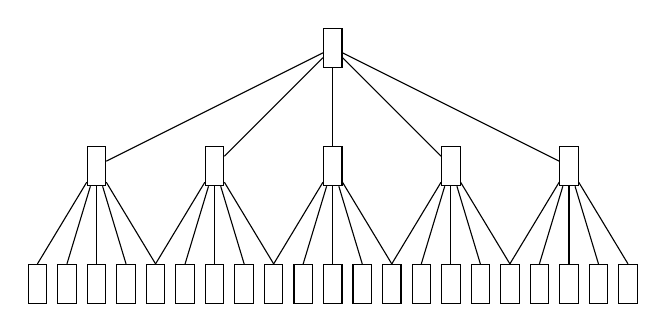
\begin{tikzpicture}[x=1.5cm, y=1.5cm, >=stealth]
    % Layers
    \foreach \m [count=\y] in {1,2,...,21}
    \node [tdnn neuron] (input-\m) at (0-\y*0.25,0) {};

    \foreach \m [count=\y] in {1,2,...,5}
    \node [tdnn neuron] (hidden-1-\m) at (0-\y*1 + 0.25,1) {};

    \foreach \m [count=\y] in {1}
    \node [tdnn neuron] (classify-\m) at (0-\y*0.25 - 10 * 0.25,2) {};

    %Edges
    \foreach \m [
    evaluate=\m as \nstart using ((\m - 1) * 4) + 1,
    evaluate=\m as \nstep using ((\m - 1) * 4) + 2,
    evaluate=\m as \nend using ((\m - 1)* 4) + 5] in {1,2,...,5}
    \foreach \i in {\nstart,\nstep,...,\nend}{
    \pgfmathparse{int(\i)}
    \draw (input-\pgfmathresult.north) -- (hidden-1-\m); % Error happens here. 
        }

    \foreach \m in {1,2,...,5}{
        \draw (hidden-1-\m) -- (classify-1);
        }
    \end{tikzpicture}
\end{frame}
\end{document}
